\section{Introduction}
In Listing \ref{c:arrayEx}, we used `$\%4d$' and `$\%21.5$' etc. to print the outputs in readable format. In this chapter, we will some more commands for formatting input and outputs i.e. `scanf' and `printf' commands respectively. 

\section{Printing Integer and Floating point values}
Table \ref{tbl:FormatIntFloat} shows the list of `conversion specifier' e.g. `d' and `f' etc. for printing `Integer' and `Floating point' values. Further, these specifiers are used to print the values in different formats in Listing \ref{c:printIntFloat}. 
\begin{table}[!h]
	\centering
	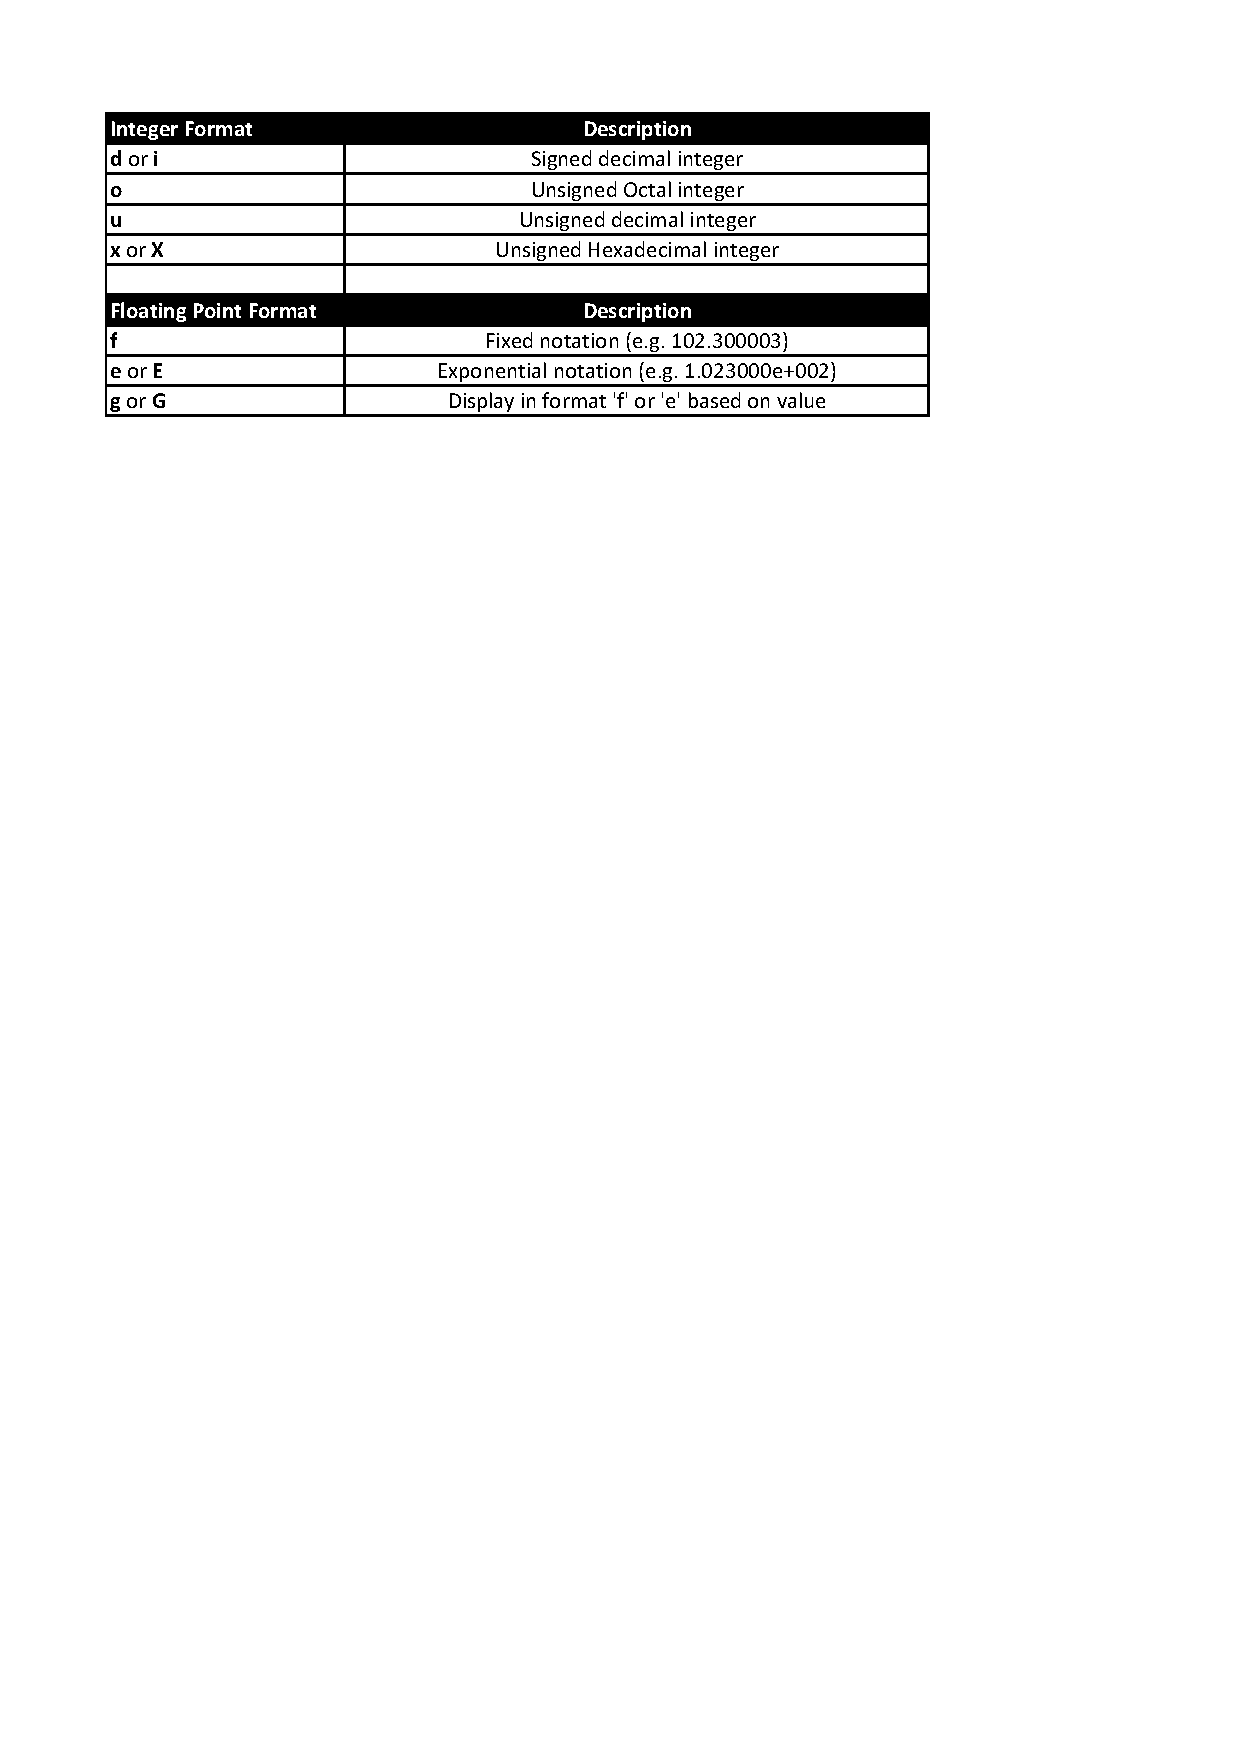
\includegraphics{FormatIntFloat}
	\caption{Print numbers in various formats}
	\label{tbl:FormatIntFloat}
\end{table}


\lstinputlisting[
language = C,
caption    = {Different formats Integer and Float values},
label      = {c:printIntFloat}
]{printIntFloat.c}

\section{Modify `printf' format}
Table \ref{tbl:printfFormat} shows various flags which can be used to format the outputs for the `printf' statement. Listing \ref{c:printfFlag} and \ref{c:printfPrefix} show the usage of these flags. Please read the comments under these listings. 
\begin{table}[!h]
	\centering
	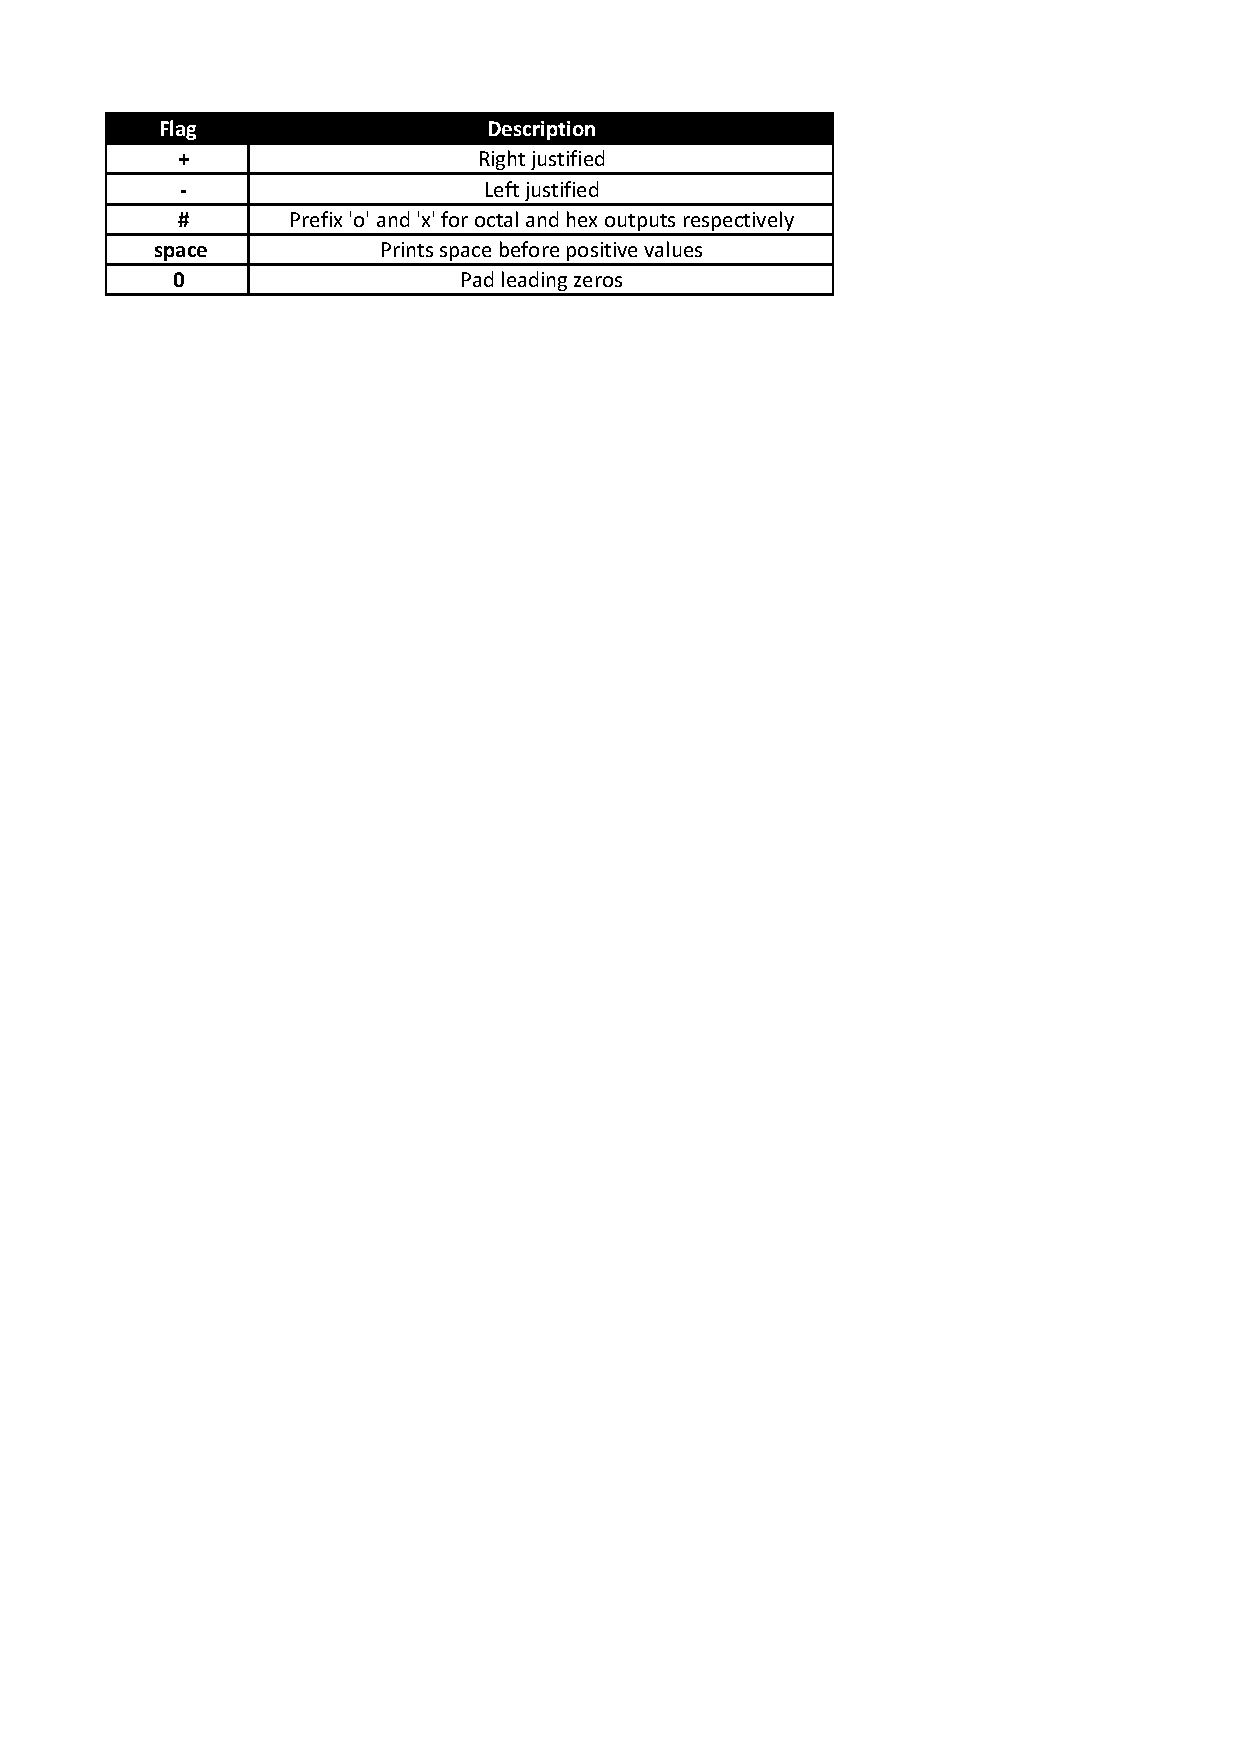
\includegraphics{printfFormat}
	\caption{`printf' formats}
	\label{tbl:printfFormat}
\end{table}

\lstinputlisting[
language = C,
caption    = {`Left \& right justified' and `signs'},
label      = {c:printfFlag}
]{printfFlag.c}

\lstinputlisting[
language = C,
caption    = {`$\#$' to print `0x' and `0' before hex and oct numbers respectively},
label      = {c:printfPrefix}
]{printfPrefix.c}

\section{Formatted input using `Scanf'}
In this section, we will see various methods to get inputs from user with `scanf' command. 

\subsection{Format specifiers}
We can use all the formats specified in Table \ref{tbl:FormatIntFloat} with `scanf' as well. \textbf{The difference is in `d' and `i' specifiers i.e. `d' can only read integer format, where `i' can read `Octal' and `Hexadecimal' formats as well, as shown in Listing \ref{c:scanfExFormat}}.

\lstinputlisting[
language = C,
caption    = {Difference in `d' and `i'},
label      = {c:scanfExFormat}
]{scanfEx.c}

\subsection{Scan and rejection set}
We can select or reject data from the input provided by user, as shown in Listing \ref{c:scanSetEx} and Listing \ref{c:invertedScanSetEx} respectively. $[ abc ]$ is used for creating the scan-set, whereas $[ \hat abc ]$ is used for rejection-set. Please see comments in the listing for better understanding. 

\lstinputlisting[
language = C,
caption    = {S\textbf{Inverted s}can set},
label      = {c:scanSetEx}
]{scanSetEx.c}

\lstinputlisting[
language = C,
caption    = {Inverted scan set},
label      = {c:invertedScanSetEx}
]{invertedScanSetEx.c}
 
\subsection{Suppression character `*'}
Suppression character can be used for removing certain characters while reading input e.g. while reading date in `dd-mm-yyyy', we can skip the `-' as shown in Listing \ref{c:suppressCharEx}, where two methods are shown for suppressing the characters. 

\lstinputlisting[
language = C,
caption    = {Suppression character},
label      = {c:suppressCharEx}
]{suppressCharEx.c}

\section{Conclusion}
In this section, we saw various methods to format the input and output data using `scanf' and `printf' command respectively. 